\section{方法描述}

\subsection{数据增广}

\subsubsection{随机重排}

在菜品预测问题中,原料的先后顺序应当与最终的菜系类别无关。因此我们对于每个输入样本,将其原料进行随机重排得到新的增广样本,如表~\ref{tab:randperm}~所示。例如``香草''、``牛奶''、``蛋黄''、``白糖''、``玉米淀粉''进行随机重排后,可能为``白糖''、``牛奶''、``蛋黄''、``玉米淀粉''、``香草''。

\begin{table}[htbp]
    \centering
    \begin{tabular}{lccccc}
        \toprule
        原始数据 & $p_1$ & $p_2$ & $p_3$ & $p_4$ & $p_5$ \\
        \midrule
        增广数据 & $p_4$ & $p_2$ & $p_3$ & $p_5$ & $p_1$ \\
        \bottomrule
    \end{tabular}
    \caption{随机重排示例}
    \label{tab:randperm}
\end{table}

\subsubsection{随机删除}

制作菜品时通常会用到多种原料,缺少一种原料往往不会影响最终的菜系类别。因此在模型训练阶段,我们随机删去每个训练样本中的一种原料,如表~\ref{tab:randdrop}~所示。例如``香草''、``牛奶''、``蛋黄''、``白糖''、``玉米淀粉''进行随机删除后,可能为``香草''、``牛奶''、``蛋黄''、``玉米淀粉''。

\begin{table}[htbp]
    \centering
    \begin{tabular}{lccccc}
        \toprule
        原始数据 & $p_1$ & $p_2$ & $p_3$ & $p_4$ & $p_5$\\
        \midrule
        增广数据 & $p_1$ & $p_2$ & $p_3$ & $p_5$ & \\
        \bottomrule
    \end{tabular}
    \caption{随机删除示例}
    \label{tab:randdrop}
\end{table}

\subsection{模型架构}

我们选用TextCNN架构\cite{kim2014convolutional}构造用于菜品预测的神经网络模型,将原料词组按顺序拼接为一个单词序列作为模型输入。假设输入序列$x$包含$n$个单词,首先将序列中每个单词$w_i$映射为$k$维的词向量$e_i\in\mathbb{R}^k$作为卷积层的输入。卷积层共包含$h$个卷积核$f\in\mathbb{R}^{mk}$,每个卷积核以$m$个连续单词作为输入,通过以下函数计算输出$c_i$:
\begin{equation}
    c_i=\text{ReLU}(f\cdot e_{i:i+m-1}+b_f)
\end{equation}
其中$b_f\in\mathbb{R}$是偏置项,我们选用修正线性单元ReLU作为非线性激活函数。

每个卷积核在整段输入序列上进行卷积,遍历所有可能的窗口$\{e_{1:m},e_{2:m+1},\ldots,e_{n-m+1:n}\}$产生特征图:
\begin{equation}
    c=[c_1,c_2,\ldots,c_{n-m+1}]
\end{equation}
其中$c\in\mathbb{R}^{n-m+1}$。

我们使用最大池化操作根据特征图计算出当前卷积核的输出:
\begin{equation}
    \hat{c}=\max_i c_i
\end{equation}

假设整个卷积层共有$h$个卷积核,我们将所有卷积核的输出拼接作为池化层的输出$q\in\mathbb{R}^h$:
\begin{equation}
    q=[\hat{c}_1,\hat{c}_2,\ldots,\hat{c}_h]
\end{equation}

最后我们使用Softmax层计算每个菜系类别的预测概率$o\in\mathbb{R}^C$:
\begin{equation}
    o=\text{Softmax}(W_oq+b_o)
\end{equation}
其中$C=20$,$W_o$和$b_o$分别为Softmax层的权重和偏置。

我们将TextCNN模型的整体架构绘制在图~\ref{fig:model}~中。

\begin{figure}[htbp]
    \centering
    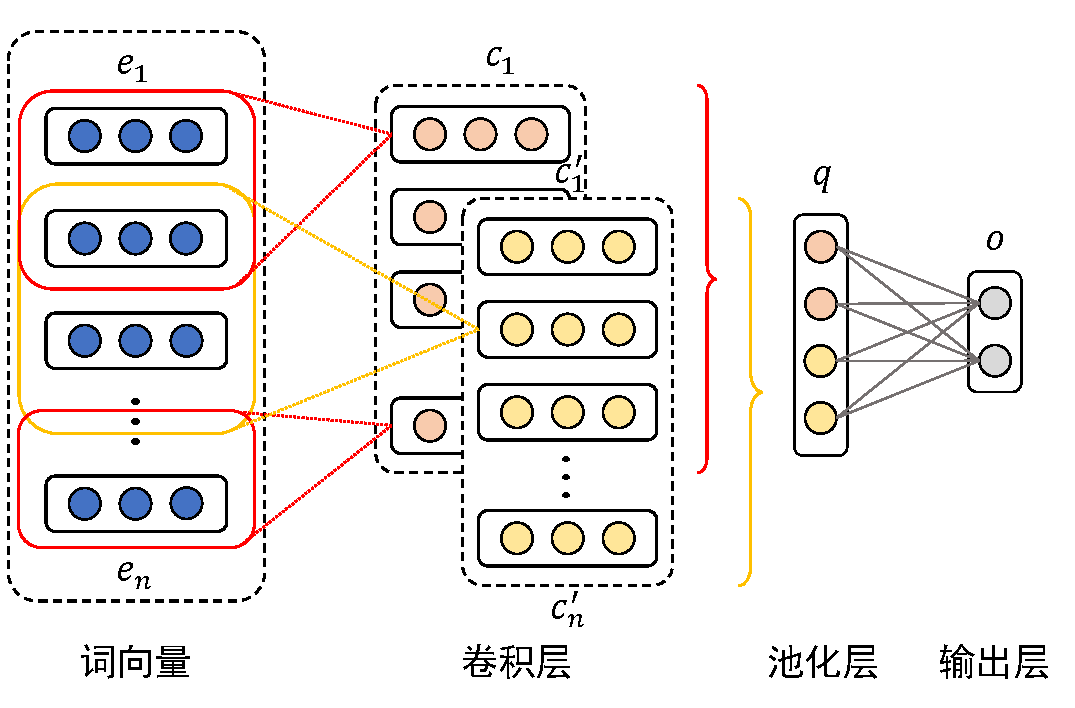
\includegraphics[width=.6\textwidth]{figs/textcnn.pdf}
    \caption{TextCNN模型架构图}
    \label{fig:model}
\end{figure}

\subsection{损失函数}

假设训练集中包含$T$个训练样本$(x_t,y_t)$。对于多分类问题,通常我们使用交叉熵损失函数来优化模型参数,同时附加权重衰减正则项:
\begin{equation}
    \mathcal{L}(\hat{y},y)=-\sum_{i=1}^T\sum_{j=1}^Cy_i^j\log(\hat{y}_i^j)+\lambda\sum_{\theta\in\Theta}\Vert\theta\Vert_2^2
\end{equation}
其中$y_i^j$代表真实类别,$\hat{y}_i^j$代表预测类别,$C=20$,$\Theta$对应全部的可训练参数,$\lambda$控制权重衰减正则项对训练过程的影响程度。
